\subsection{Ở phạm vi con người}
	Trước khi trả lời câu hỏi này, hãy khảo sát sơ qua ý tưởng ứng dụng thuật toán di truyền vào mạng Neural Network bằng cách đặt câu hỏi trong bối cảnh con người chúng ta.
	
	Không thể phủ nhận rằng, con người là một bản thể sinh học có sự sống, mỗi cá thể trong quần thể con người đều có những đặc điểm riêng đầy thú vị. Dựa trên lí giải sinh học, ta biết rằng chính gen là bộ khung tạo nên và làm cho quần thể con người tồn tại nhiều cá thể đầy thú vị.
	
	Và thú vị hơn nữa, mỗi chúng ta đều có một tư duy khác nhau và độc lập với người khác. Ở điểm này, vậy có phải di truyền cũng là thứ làm cho chúng ta khác biệt ở nhận thức? Đây là một câu hỏi mà để trả lời nó cần giao thoa quan điểm của nhiều thứ (di truyền, môi trường, xã hội, biến cố, …), song không thể gạt bỏ di truyền ra khỏi tư duy.
	
	Theo dòng chảy của suy luận trên, ta biết di truyền có kết nối với tư duy. Dựa trên mối kế thừa quan hệ ở lập trình, ta cũng phần nào đoán nhận giải thuật di truyền phải có một kết nối gì đó đến Neural Network.
	
	\begin{figure}[h]
		\centering
		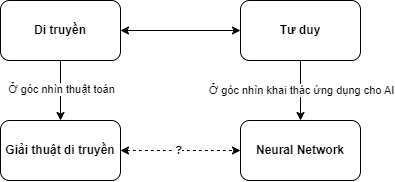
\includegraphics{figures/thought_and_genetic.png}
		\caption{Sơ đồ trên thể hiện Di truyền và tư duy có mối quan hệ với nhau. Thông qua góc nhìn thuật toán đối với di truyền làm phát sinh giải thuật di truyền, góc nhìn khai thác ứng dụng AI làm cho phát sinh mạng thần kinh nhân tạo (ANN). Mặt khác di truyền và tư duy có mối quan hệ, vậy thì giải thuật di truyền và ANN cũng phải có quan hệ tương tự. Dấu ? tượng trưng cho việc chưa xác định được mối quan hệ đó là gì.}
		\label{fig:thought_and_genetic}
	\end{figure}
	
\subsection{Thử khai thác dấu ?}
	Đặt mục tiêu khai thác trong bối cảnh mạng FNN, ta thấy FNN có một số điểm đáng lưu tâm như sau:
	\begin{itemize}
		\item Kiến trúc FNN. Đó là số lượng số đơn vị neuron, số tầng, hàm kích hoạt, số tham số.
		\item Tham số FNN. Là về các trọng số kết nối giữa các tầng. 
	\end{itemize}
	
	Mặt khác, một quy trình ứng dụng của mạng FNN gồm hai pha cơ bản sau:
	\begin{itemize}
		\item Pha đào tạo (Training). Là pha học của mạng. Là pha thay đổi các tham số sao cho việc chuyển đổi giữa X (Input) sang Y (Output) là tốt nhất có thể. \cite{kak1993training}
		\item Pha ứng dụng. Là pha khai thác mạng đã qua đào tạo, đem vào dùng với dữ liệu có thể chưa qua đào tạo.
	\end{itemize}
	
	Xét đến, thuật toán di truyền (Genetic Algorithm) là một thuật toán tối ưu. Tuân theo quy trình, ta nắm được GA sẽ tham gia vào pha đào tạo (Training). Xét đến những điểm đáng lưu tâm, ta khẳng định GA có thể dùng để tối ưu các thành phần của mô hình như kiến trúc và tham số. \cite{montana1989training}
	
\noindent

Đối với các mô hình AI hiện tại, thường việc tối ưu sẽ dựa trên các phương pháp liên quan đến Gradient. Thuật toán di truyền nói riêng và họ thuật toán tối ưu không dùng Gradient vẫn đang phát triển nhưng không nổi trội bằng nhánh trên.